\documentclass[sigconf]{acmart}
\usepackage{amsmath}
\settopmatter{printacmref=false}

%% remove copyright and further ACM refs for the Lab
\setcopyright{none}
\copyrightyear{}
\acmDOI{}
\acmISBN{}
\acmConference[Data Science Lab]{Data Science Lab}{2021}{Uni Passau}

%% end of the preamble, start of the body of the document source.
\begin{document}

%%
%% The "title" command has an optional parameter,
%% allowing the author to define a "short title" to be used in page headers.
\title{A Report of Trajectory Prediction based on Deep Learning}

%% author list and team

\author{Chenxiao Tian}
\email{tian01@ads.uni-passau.de}
\affiliation{\institution{University of Passau}}

\author{Rita Akhmetova}
\email{akhmet01@ads.uni-passau.de}
\affiliation{\institution{University of Passau}}

\author{Yashu Wang}
\email{wang52@ads.uni-passau.de}
\affiliation{\institution{University of Passau}}

\author{Zubair Ahmed}
\email{ahmed08@ads.uni-passau.de}
\affiliation{\institution{University of Passau}}

\renewcommand{\shortauthors}{team 4: Trajectory Prediction}

\begin{abstract}
    Pedestrians trajectory prediction has received significant importance over the last few years due to the increase in autonomous robots and vehicles, specifically in the automotive industry because of the rising number of self-driving vehicles. Different methods can be used to accomplish the trajectory prediction task. In recent years, GANs (Generative Adversarial Networks) have been applied to trajectory prediction because of their good multimodal performance. However, GANs also introduce a latent space, which is completely unknown and uncontrollable. In this report, we tried to overcome this problem by InfoGAN (an information-theoretic extension of Generative Adversarial Network). Our InfoGAN implementation attempts to learn a disentangled representation of plausible future trajectories in a completely unsupervised manner. In addition, we added a regularization to constrain that changes in different codes should be uncorrelated and disentangled a factor that can move the trajectory upwards/downwards.
\end{abstract}

%%
%% This command processes the author and affiliation and title
%% information and builds the first part of the formatted document.
\maketitle
\section*{Phases Assignment}
\begin{itemize}
    \item \textbf{Phase1} \emph{Chenxiao Tian}
    \item \textbf{Phase2} \emph{Zubair Ahmed}
    \item \textbf{Phase3} \emph{Yashu Wang}
    \item \textbf{Phase4} \emph{Rita Akhmetova}
\end{itemize}


\section*{Introduction}
The innate abilities that human beings possess to process complex things effortlessly in daily life are impressive. To translate even the fractional part of one of these abilities of the human being into a machine is a challenging task in itself. One such ability is to navigate in a social environment. For example, when we walk in a crowded public space we follow a large number of common-sense rules and social etiquette. Which includes respecting the personal space of others, yielding right-of-way, avoiding walking through the people belonging to the same group, taking the shortest path or safer path to the destination, and much more.

This ability of ours in the field of technology is known as Human/pedestrian trajectory prediction. The task of predicting human trajectories for machines is very important in current and future advancements. Many end-user applications make intensive use of data analytics about pedestrians motion: urban safety, city planning, marketing, autonomous driving, to name a few. Typically, this implies the recollection and the offline analysis of these data, for understanding the pedestrian's behavior and taking decisions about the environment.
In some contexts, however, one needs to go further and anticipate, in an online way, what will be the next pedestrian moves and infer their short or mid-term intentions. This allows to trigger early alarms or to take preventive actions when monitoring systems with critical real-time decision-making processes. In the case of autonomous driving, for example, inferring the intention of the pedestrians surrounding the car is of paramount importance in avoiding collisions. Many researches have proposed miscellaneous approaches that tackle this problem. Helbing and Molnar~\cite{Helbing95} propose the Social Force model. Yi~\cite{Yi15} introduces the factor of stationary group to the modeling of pedestrians trajectories with an energy map. The aforementioned ways are deterministic ways for prediction, they can not utilize the valuable information in the trajectories data.

Over the last few years, following the widespread usage of machine learning and deep learning methods, researchers use various neural networks to tackle the trajectories prediction problem. Zhou et al.~\cite{Zhou} build a linear dynamic system, applying Expectation Maximization (EM) algorithm to estimate parameters, to learn motion patterns in crowded scenes. Altché~\cite{Altche17} proposes a method that predicts the trajectory on the highway using Long Short-Term Memory (LSTM). Alahi et al.~\cite{Alahi16} give a sequence model based on LSTM as well as a social pooling that aggregates the human-human interaction in a scene.

However, these approaches mentioned previously learn only the pattern of human motion from data. Predicting human trajectory is a complex task. This is because both internal and external stimuli, such as intentions and other directly or indirectly observable influences, can affect human motion, as mentioned in the survey~\cite{humanmotionsurvey}. In addition to the location, which is usually recorded in the dataset, many factors that are not explicitly recorded in the dataset, such as speed, direction, or even not recorded, such as route and human intent. Recent researches have shown that Generative Adversarial Network (GAN) can better capture these uncertainties with latent space and thus naturally preserve multimodality. Gupta et al.~\cite{Gupta_2018_CVPR} used GAN and a Pooling Module to predict socially acceptable trajectories and found that certain directions in the latent space are related to direction and velocity. What is more, the study of Amirian et al.~\cite{Amirian_2019_CVPR_Workshops} has shown that InfoGAN, an information-theoretic extension to the Generative Adversarial Network~\cite{infogan}, partly improves the performance on commonly used datasets that have the largest variance in the prediction distribution, while still leaving some room for improvement.

Even though these researches give various effective models that fulfill the prediction task and attempt to encompass hidden aspects that influence the trajectory, they have not disentangled these factors in the latent space. If we know the factors that affect pedestrians' trajectory and apply these factors in specific scenarios, we can obtain better performance of prediction on various distributed datasets and to mitigate the limitations of the observed data. Therefore, we decide to consider the hidden factors behind different datasets.

In this study, we focus on what factors we can obtain that influence human trajectories and try to develop a model that can be controlled by these factors. we assume that different datasets have different static environments and so the data in a dataset share some specific common features. We consider three factors: obstacles (obstacles information such as the presence of static obstacles and the coordinates), maps (geometry and topology), and semantics (environment semantics such as no-go-zones, crosswalks, sidewalks, or traffic lights) in static environments, which are denoted by the survey~\cite{humanmotionsurvey}. We propose to develop a controllable generation model that is controlled by factor $c$ to have different static environments. We demonstrate that human movement is influenced by these three factors that we consider in a static environment. Also, with inputting different factors in static environments, our model can achieve better performance on different datasets.

\section{Problem Statement}
In this paper, our goal is to develop a controllable generative model to predict pedestrian trajectories.
Consider the problem of predicting the future trajectory of each pedestrian. Let $(x_i^t, y_i^t)$ denote the position of the $i$ pedestrian at time $t$, and a sequence of coordinates  $[(x_i^{t}, y_i^{t}), (x_i^{t+1}, y_i^{t+1}), ..., (x_i^{t+n}, y_i^{t+n})]$ denote the trajectory of pedestrians from time $t$ to $t+n$.

Given the observed trajectory of $n_{obs}$ steps $X_i^t = [(x_i^{t}, y_i^{t}), \\ (x_i^{t+1}, y_i^{t+1}), ..., (x_i^{t+n_{obs}}, y_i^{t+n_{obs}})]$, with certain controllable factor $c$ and random variable $z$,  we want to fit a function to generate the prediction of trajectory for the next $n_{pred}$ steps $Y_i^t = [(x_i^{t+n_{obs}+1}, \\  y_i^{t+n_{obs}+1}), (x_i^{t+n_{obs}+ 2}, y_i^{t+n_{obs}+2}), ...,  (x_i^{t+n_{obs}+ n_{pred}}, y_i^{t+n_{obs}+n_{pred}})]$. That is
$$ Y_i^t = f(X_i^t \vert c, z) $$

The prediction $Y_i^t$ is controllable by the vector $c$, where consist of $(c_1, c_2, c_3)$. So we can control the factors of obstacles, maps, and semantics respectively. These factors are independent of each other. They may vary depending on the data set and time.


\section{Data Acquisition \& Pre-Processing}
This section discusses the dataset used for pedestrian trajectory prediction. Since the trajectory prediction is a data-driven task, and the data-driven task requires its data to be available in quantity with sufficient quality. Data for pedestrian trajectory prediction can be obtained in two different formats: either in image coordinates or in real-world coordinates. Image coordinates mean that each pedestrian is represented with the pixels it occupies in an image from the camera, whereas real-world coordinates mean that each pedestrian is represented by its position in meters (basic metric unit of length) with origin in an arbitrary point of the world.\newline
The choice of the coordinate format selection depends on the type of the application: image coordinates are mostly used in video surveillance applications, whereas real-world coordinates are used in autonomous driving, robotic, or other similar applications. As we focus on the prediction of pedestrian trajectory in real-world scenarios therefore our datasets are using real-world coordinates.\newline
Since acquiring new data for the research is a very difficult and expensive task. Often ETH and UCY are the most commonly used datasets in different research works, due to their public availability and use of real-world coordinates. Hence we are also using the ETH and UCY datasets in this research.

\subsection{Data acquisition}
The most commonly used datasets for pedestrian trajectory prediction are ETH and UCY datasets.
The BIWI Walking Pedestrians (also named ETH Walking Pedestrians [EWAP]) dataset referred to as ETH \cite[]{ETH-biwi} is the research work of Pellegrini et al. from ETH Zurich University, this dataset is comprised of two scenes (namely eth and hotel) taken from a bird's eye view. In total the dataset has 785 different pedestrians 365 and 420 for eth and hotel respectively. The pedestrian position is annotated at 2.5fps in both datasets that is every 0.4 seconds of a trajectory. Figure \ref{fig:eth-dataset-scenes} represents each scenes from the ETH dataset.\newline
Whereas the UCY dataset \cite[]{UCY-crowds} is the research work of Lerner et al. from the University of Cyprus. The dataset is comprised of three scenes (univ, zara1, and zara2), also taken from a bird's eye view. In total it contains trajectories of more than 1100 pedestrians containing 850, 148, and 204 for univ, zara1, and zara2 respectively. Just like ETH, the UCY dataset is also annotated with pedestrian positions every 0.4 seconds. Figure \ref{fig:crowds-dataset-scenes} represents each scences from the UCY dataset.\newline
These two datasets are often used in combination: in total, they contain five scenes (eth, hotel, univ, zara1, and zara2), with more than 1800 pedestrian trajectories. For training and testing purposes we use leave-one-out approach: basically, the model is first trained on four scenes and tested on the fifth, and the procedure is repeated five times, once for each scene.\newline 
The original datasets can be downloaded directly from the official download links (ETH - BIWI Walking Pedestrians dataset)~\footnote{\label{fn:eth-dataset}\url{https://data.vision.ee.ethz.ch/cvl/aem/ewap_dataset_full.tgz}}, and (UCY - Crowded Data)~\footnote{\label{fn:ucy-dataset}\url{https://graphics.cs.ucy.ac.cy/research/downloads/crowd-data}}.

\begin{figure}[h]
  \centering
  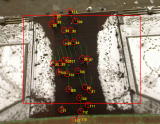
\includegraphics[width=0.40\linewidth]{./figures/image-biwi.png}
  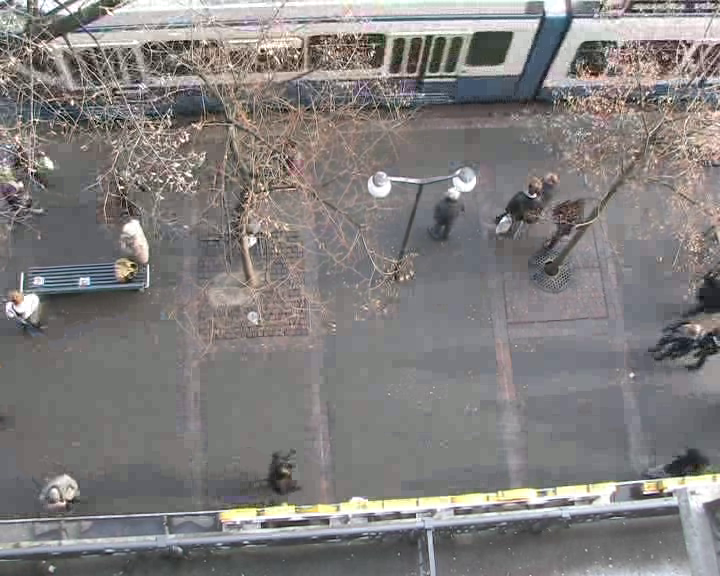
\includegraphics[width=0.40\linewidth]{./figures/biwi-hotel.png}
  \caption{EWAP$^{\ref{fn:eth-dataset}}$ datasets scenes - left image represents scene from eth, while right from hotel dataset \cite[]{UCY-crowds}.}\label{fig:eth-dataset-scenes}
  \Description{ETH dataset images}
\end{figure}

\begin{figure}[h]
  \centering
  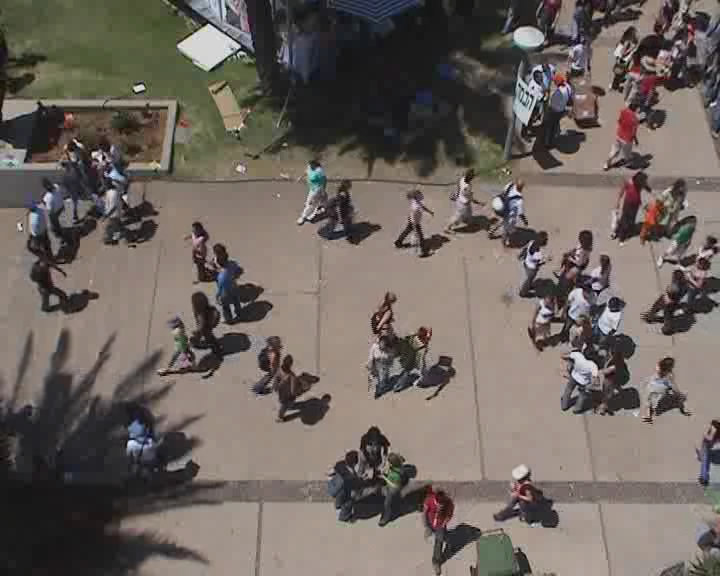
\includegraphics[width=0.40\linewidth]{./figures/students_003.jpg}
  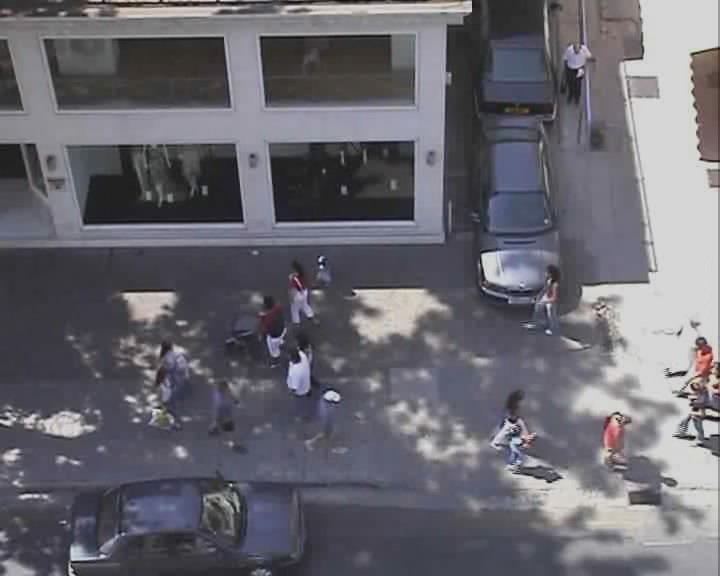
\includegraphics[width=0.40\linewidth]{./figures/crowds_zara01.jpg} % crowds_zara2.jpg is same
  \caption{UCY$^{\ref{fn:ucy-dataset}}$ datasets scenes - left image represents scene from univ, while right image from zara1 and zara2 dataset \cite[]{ETH-biwi}.}\label{fig:crowds-dataset-scenes}
  \Description{UCY crowds dataset images}
\end{figure}

\subsection{Data preprocessing}
In this research, we use ETH and UCY datasets for the implementation of InfoGAN based trajectory prediction model. The dataset that is available from ETH is provided in a text file where each line represents frame number in the scene, pedestrian id, pedestrian positions, and velocities in x y z coordinates in the respective frame, the data is formatted as:
\begin{center}
  [frame\char`_number, pedestrian\char`_ID, pos\char`_x, pos\char`_z, pos\char`_y, v\char`_x, v\char`_z, v\char`_y]
\end{center}
The metric used is `meters' for the positions and velocities. The dataset also includes the homography matrix used to calculate the metric in real-world coordinates. However, pos\char`_z and v\char`_z (direction perpendicular to the ground) are not used. The data from the ETH is enough for the modeling and does not need preprocessing for our research, other than rescaling (min-max normalization).\newline
The dataset available from UCY is however uses different formatting, which requires preprocessing to format it to ETH dataset. However, we consider it to be out of the scope of this research and hence we directly use the UCY data provided by the SocialWays\cite[]{DBLP:journals/corr/ChenDHSSA16} available via a publicly shared Link~\footnote{\url{http://www.dropbox.com/sh/lh1s41d1pqp8cbx/AAD4sB1JAiZIkCL7LHht-S4Ca}} preprocessed to match the ETH dataset format.


% Phase - 3
% (uncomment below two lines for your work and use the specific file to add material)
\section{Modelling}
Our experiments are based on Social Ways. A major change in Social Ways compared to previously implemented GAN models for trajectory prediction is that it implements the InfoGAN architecture. The results from Social Ways~\cite{DBLP:journals/corr/abs-1904-09507} show that InfoGAN can greatly improve the trajectory prediction of multimodal pedestrians, avoiding pattern collapse and degradation. Figure 2 illustrates the architecture.


In the following subsections, we will describe the key methods of Social Ways and our experiments.

\subsection{Methodology}


\subsubsection{Generative Adversarial Networks}
\hfill \\
According to the research of Generative Adversarial Nets~\cite{gan}: a Generative Adversarial Network (GAN) consists of two network components, a discriminator $D$ and a generator $G$, which compete with each other. $G$ takes the input noise variable $z$ and generates the sample $G(z)$, $D$ takes the generated sample or training data as input $x$ and predicts the probability $D(x)$ that $x$ comes from the data and not generated by $G$. $D$ is trained to maximize the probability of assigning correct labels to training samples and generated samples, while $G$ is trained to minimize the correctness of $D$. In other words, $D$ and $G$ play a min-max game with the value function $V(G, D)$.

\begin{multline}
  \min_{G} \max_{D} V(G, D) = \mathbb{E}_{x \sim p_{\text{data}}} \lbrack \log(D(x))\rbrack \\ + \mathbb{E}_{z \sim p_{z}(z)} \lbrack \log(1 - D(G(z))) \rbrack
\end{multline}

In our case, for pedestrian trajectory data, the generator is trained to generate possible future trajectories that have a distribution similar to the training data, given certain previously observed trajectories, while the discriminator learns to distinguish the rationality of the generated paths. These two networks are trained simultaneously. As the discriminators are learned, the generators are improved.

\subsubsection{InfoGAN}

\hfill \\
The algorithm InfoGAN bases on Generative Adversarial Network(GAN). Even though Generator of GAN can generate fake examples from the noise input \(\mathbf{z}\), this noise vector is entangled. In other words, we can not deduce any information from the input noise vector and can not control the output of the Generator. What the data the Generator will produce is totally random. Based on GAN, InfoGAN is a way that learning interpretable representation by information. It can deduce meaningful information from the input data. Instead of using single noise input, InfoGAN accepts another input which is called latent code \(\mathbf{c}\). This latent code can be discrete or continuous. When it is discrete, a integer vector can be used to represent different factors. During training, the vector should be encoded by one hot code. Generator also contains another neural network Q which is called auxiliary network. It takes the fake data that generated by G and output the decoded latent code \( \mathbf{\hat{c}}\). By maximizing the mutual information between \( G(\mathbf{z, c})\) and \( \mathbf{\hat{c}}\), G and Q are trained. The system structure of InfoGAN is in \ref{infoGan}. The min-max game of InfoGAN is a game with the value function\cite{infogan}:
\[\min_{G,Q}\max_{D} \mathbf{V_{InfoGAN}}(D, G, Q) = \mathbf{V}_{D, G} - \lambda \mathcal{L_I}(G,Q),\] where \(\mathcal{L_I}(G,Q)\) is the lower bound of the mutual information \(\mathbf{I}(c;G(z,c))\).
\begin{figure*}[h]
  \centering
  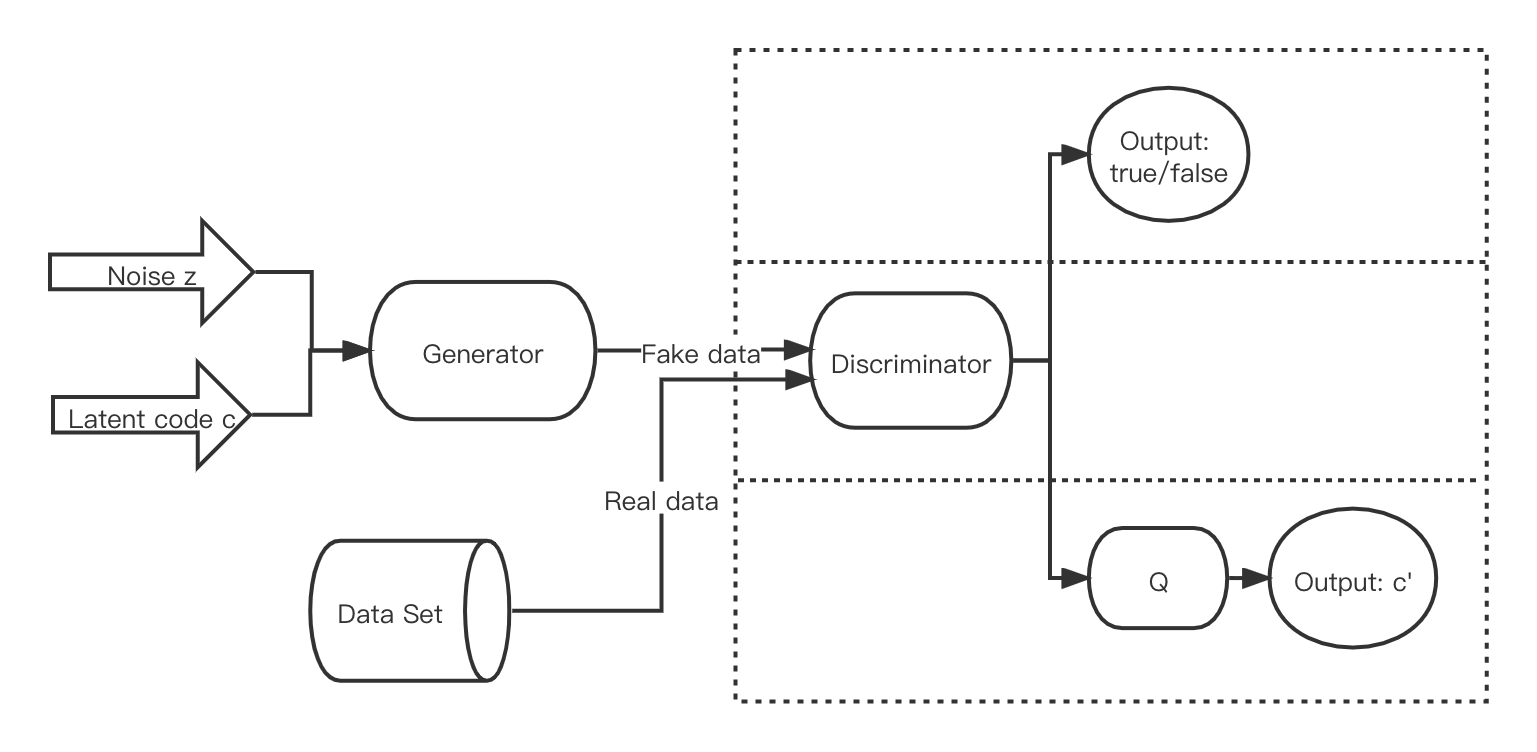
\includegraphics[width=\textwidth, height = 7cm]{figures/infoGAN.png}
  \caption{InfoGAN Overview}{InfoGAN consists of three parts, Generator G, Discriminator D and auxiliary network Q. D and Q share the network, only their last layers are different.}
%   \Description{InfoGAN consists of 3 parts, Generator G, Discriminator D and auxiliary network Q. D and Q share the network, only their last layers are different.}
  \label{infoGan}
\end{figure*}
\subsubsection{Description of Latent Code}

\hfill \\
Our experiments attempt to disentangle the latent code so that the latent code can correspond to the semantic features of the data. To enrich our expression, we allow two types of latent codes, categorical latent codes and continuous latent codes.

For categorical latent code $c$, we can use cross entropy as a loss function to maximize the information between the code and the code predicted by $Q$.


$$\mathcal{L} (c, Q(G(x, c))) = MSE(c, Q(G(x, c))) $$

For a continuous latent code $c$, we can use the mean squared error as a loss function to maximize the information between the code and the code predicted by $Q$.

$$\mathcal{L} (c, Q(G(x, c))) = CE(c, Q(G(x, c))) $$

On the basis of categorical latent codes and continuous latent codes, we can introduce a series of semantic factors. For example, velocity and direction can be represented as continuous latent codes and scenes can be expressed as categorical latent codes. For map/obstacle information, the image embedding of the background image (the background image of the video recording trajectory data) can be used as a sequence of continuous latent codes.

\subsubsection{Experimental Setup}

\hfill \\
In our project, we will train the model using three integer latent codes and three continuous latent codes. At every loop of the training of G, we modify the noise vector as the combination of an one-hot encoded vector with three random integer numbers and another vector with three random float numbers.

After the model is trained, we need to evaluate the latent codes by the method called latent traversal. Assume the discrete codes are \(\mathbf{C_1} = c_1, c_2, c_3\) and the continuous codes are  \(\mathbf{C_2}= c_4, c_5, c_6\). First we fix \(\mathbf{C_2}\) and set \(c_1 = 1, c_2 = 0, c_3=0\), then use the trained G to generate 10 trajectories. Then we draw 10 samples from the generated examples and plot the trajectories as pictures \(Pic_1\). Then fix \(\mathbf{C_2}\) and set \(c_1=0, c_2 = 1, c_3 = 0\) and generate 100 trajectories and take random 10 plot as pictures. We conduct the same process to each integer variables. Then we observe the trajectories in the picture and infer the possible factor that affects the trajectories. Our guess is speed and direction. We can start inferring  from these two factors. If we can find out the pattern in the trajectories, we can match them to the vector of integer latent codes. When evaluate the continuous codes, just fix the other two codes and change the one that is being evaluated by 0.1 every loop, the value of the code value should be in [0.1, 0.3, 0.5, 0.7, 0.9]. There will be \(3 \times 5 = 15\) groups of pictures. We observe the picture and try to deduce the factors from the trajectories.

% Phase - 4
% (uncomment below two lines for your work and use the specific file to add material)
% \section*{Evaluation}
% \subsection{Results}

In this section, we show the results of our experiments. We first show the base overview of ADE/FDE compared with baseline SGAN-20V-20.

\subsubsection{Impact of InfoGAN}

\begin{table}[ht]
  \centering
  \caption{base overview of ADE and FDE} 
  \begin{tabular}{cccc}
  \toprule
  & Dataset & SGAN + InfoGAN &  SGAN \\
  \midrule
  \multirow{5}{*}{\bf ADE} & ETH & 0.57 / 0.67 & 0.58 / 0.71 \\
                         & HOTEL & 0.30 / 0.42 & 0.36 / 0.48 \\
                         & UNIV & 0.33 / 0.54 & 0.33 / 0.56 \\
                         & ZARA1 & 0.21 / 0.34 & 0.21 / 0.34 \\
                         & ZARA2 & 0.20 / 0.31  & 0.21 / 0.31 \\
  \hline
  \multirow{5}{*}{\bf FDE} & ETH & 1.14 / 1.28 & 1.13 / 1.29 \\
                        & HOTEL & 0.57 / 0.85 & 0.71 / 1.02 \\
                        & UNIV & 0.68 / 1.14 & 0.70 / 1.18 \\
                        & ZARA1 & 0.41 / 0.70 & 0.42 / 0.69 \\
                        & ZARA2 & 0.41 / 0.64  & 0.42 / 0.64 \\

  \bottomrule
  \end{tabular}
  \label{table:adefde}
\end{table}
\hfill \\
\begin{figure}[b]
  \centering
  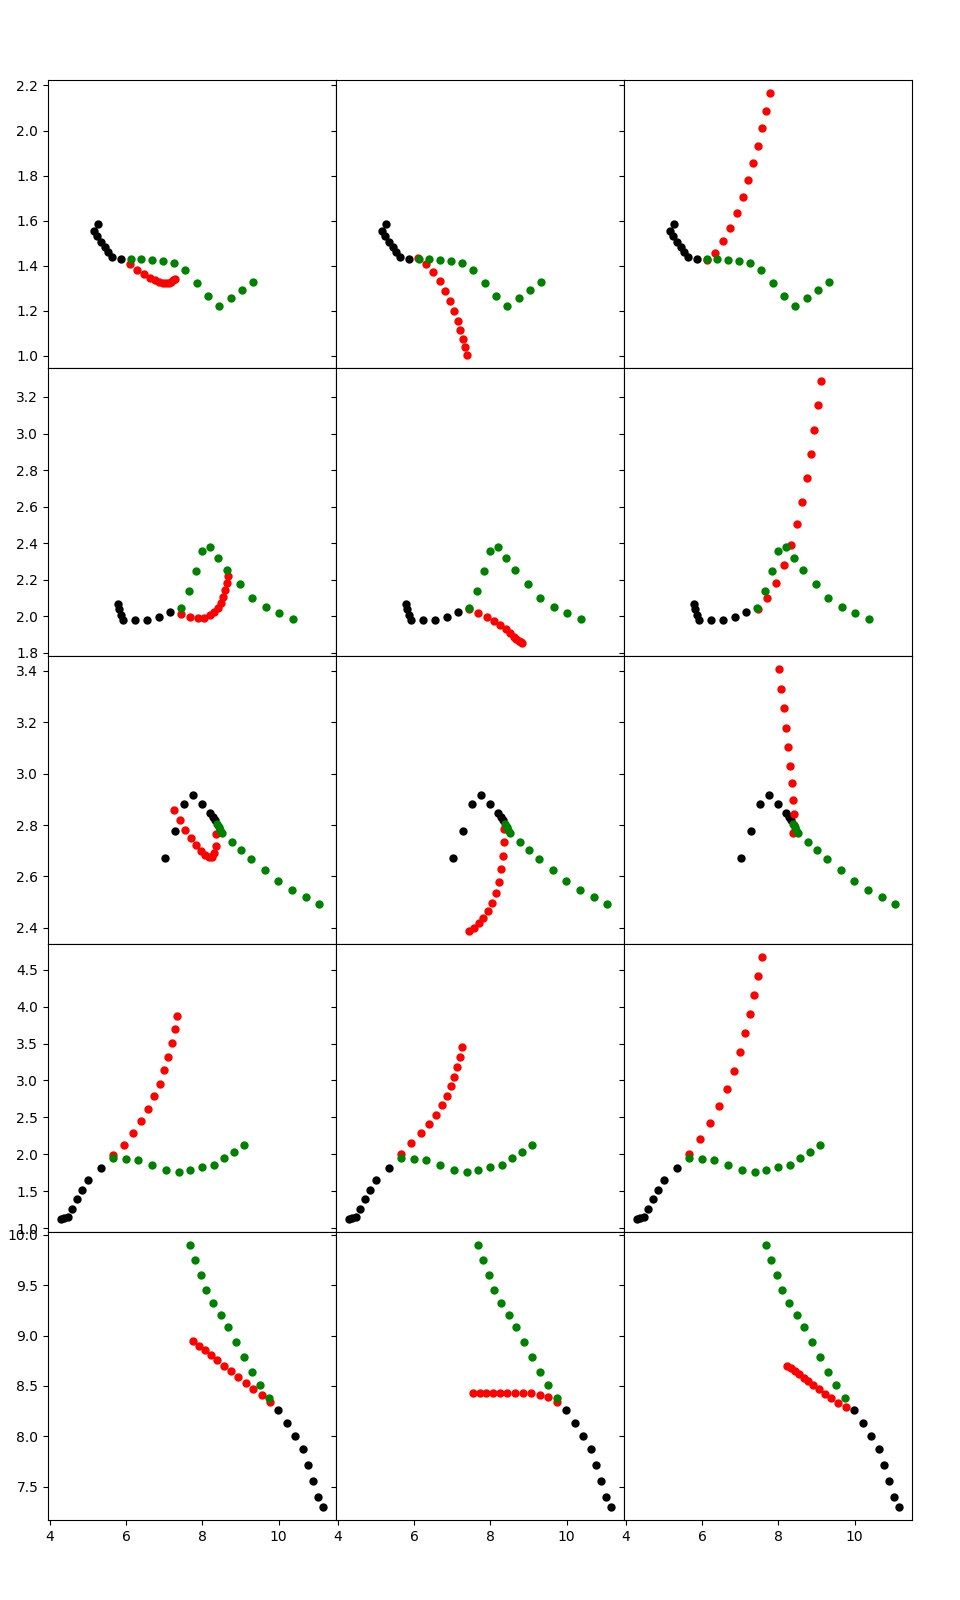
\includegraphics[width=0.3\textwidth]{figures/disc_interpolations_code0_batch2.jpeg}
  \caption{Latent traversals of three dimensional categorical code for model UNIV\_12. \normalfont{The x-axis is the traversals of three dimensions, The y-axis is the different samples. The black dots show the observed trajectory, the green dots show the ground true of the next 12 steps trajectory, the red dots show the prediction of our model.}}{Categorical latent code shows some kinds of consistent but not always(e.g. the second dimensions). More importantly, It is vary hard to  interpret the semantic meaning of the code (e.g. it is difficult to relate changes in all three dimensions to any factor.).}
  \Description{latent traversals disc code}
  \label{disc_code}
\end{figure}

\begin{figure*}[ht]
  \centering
  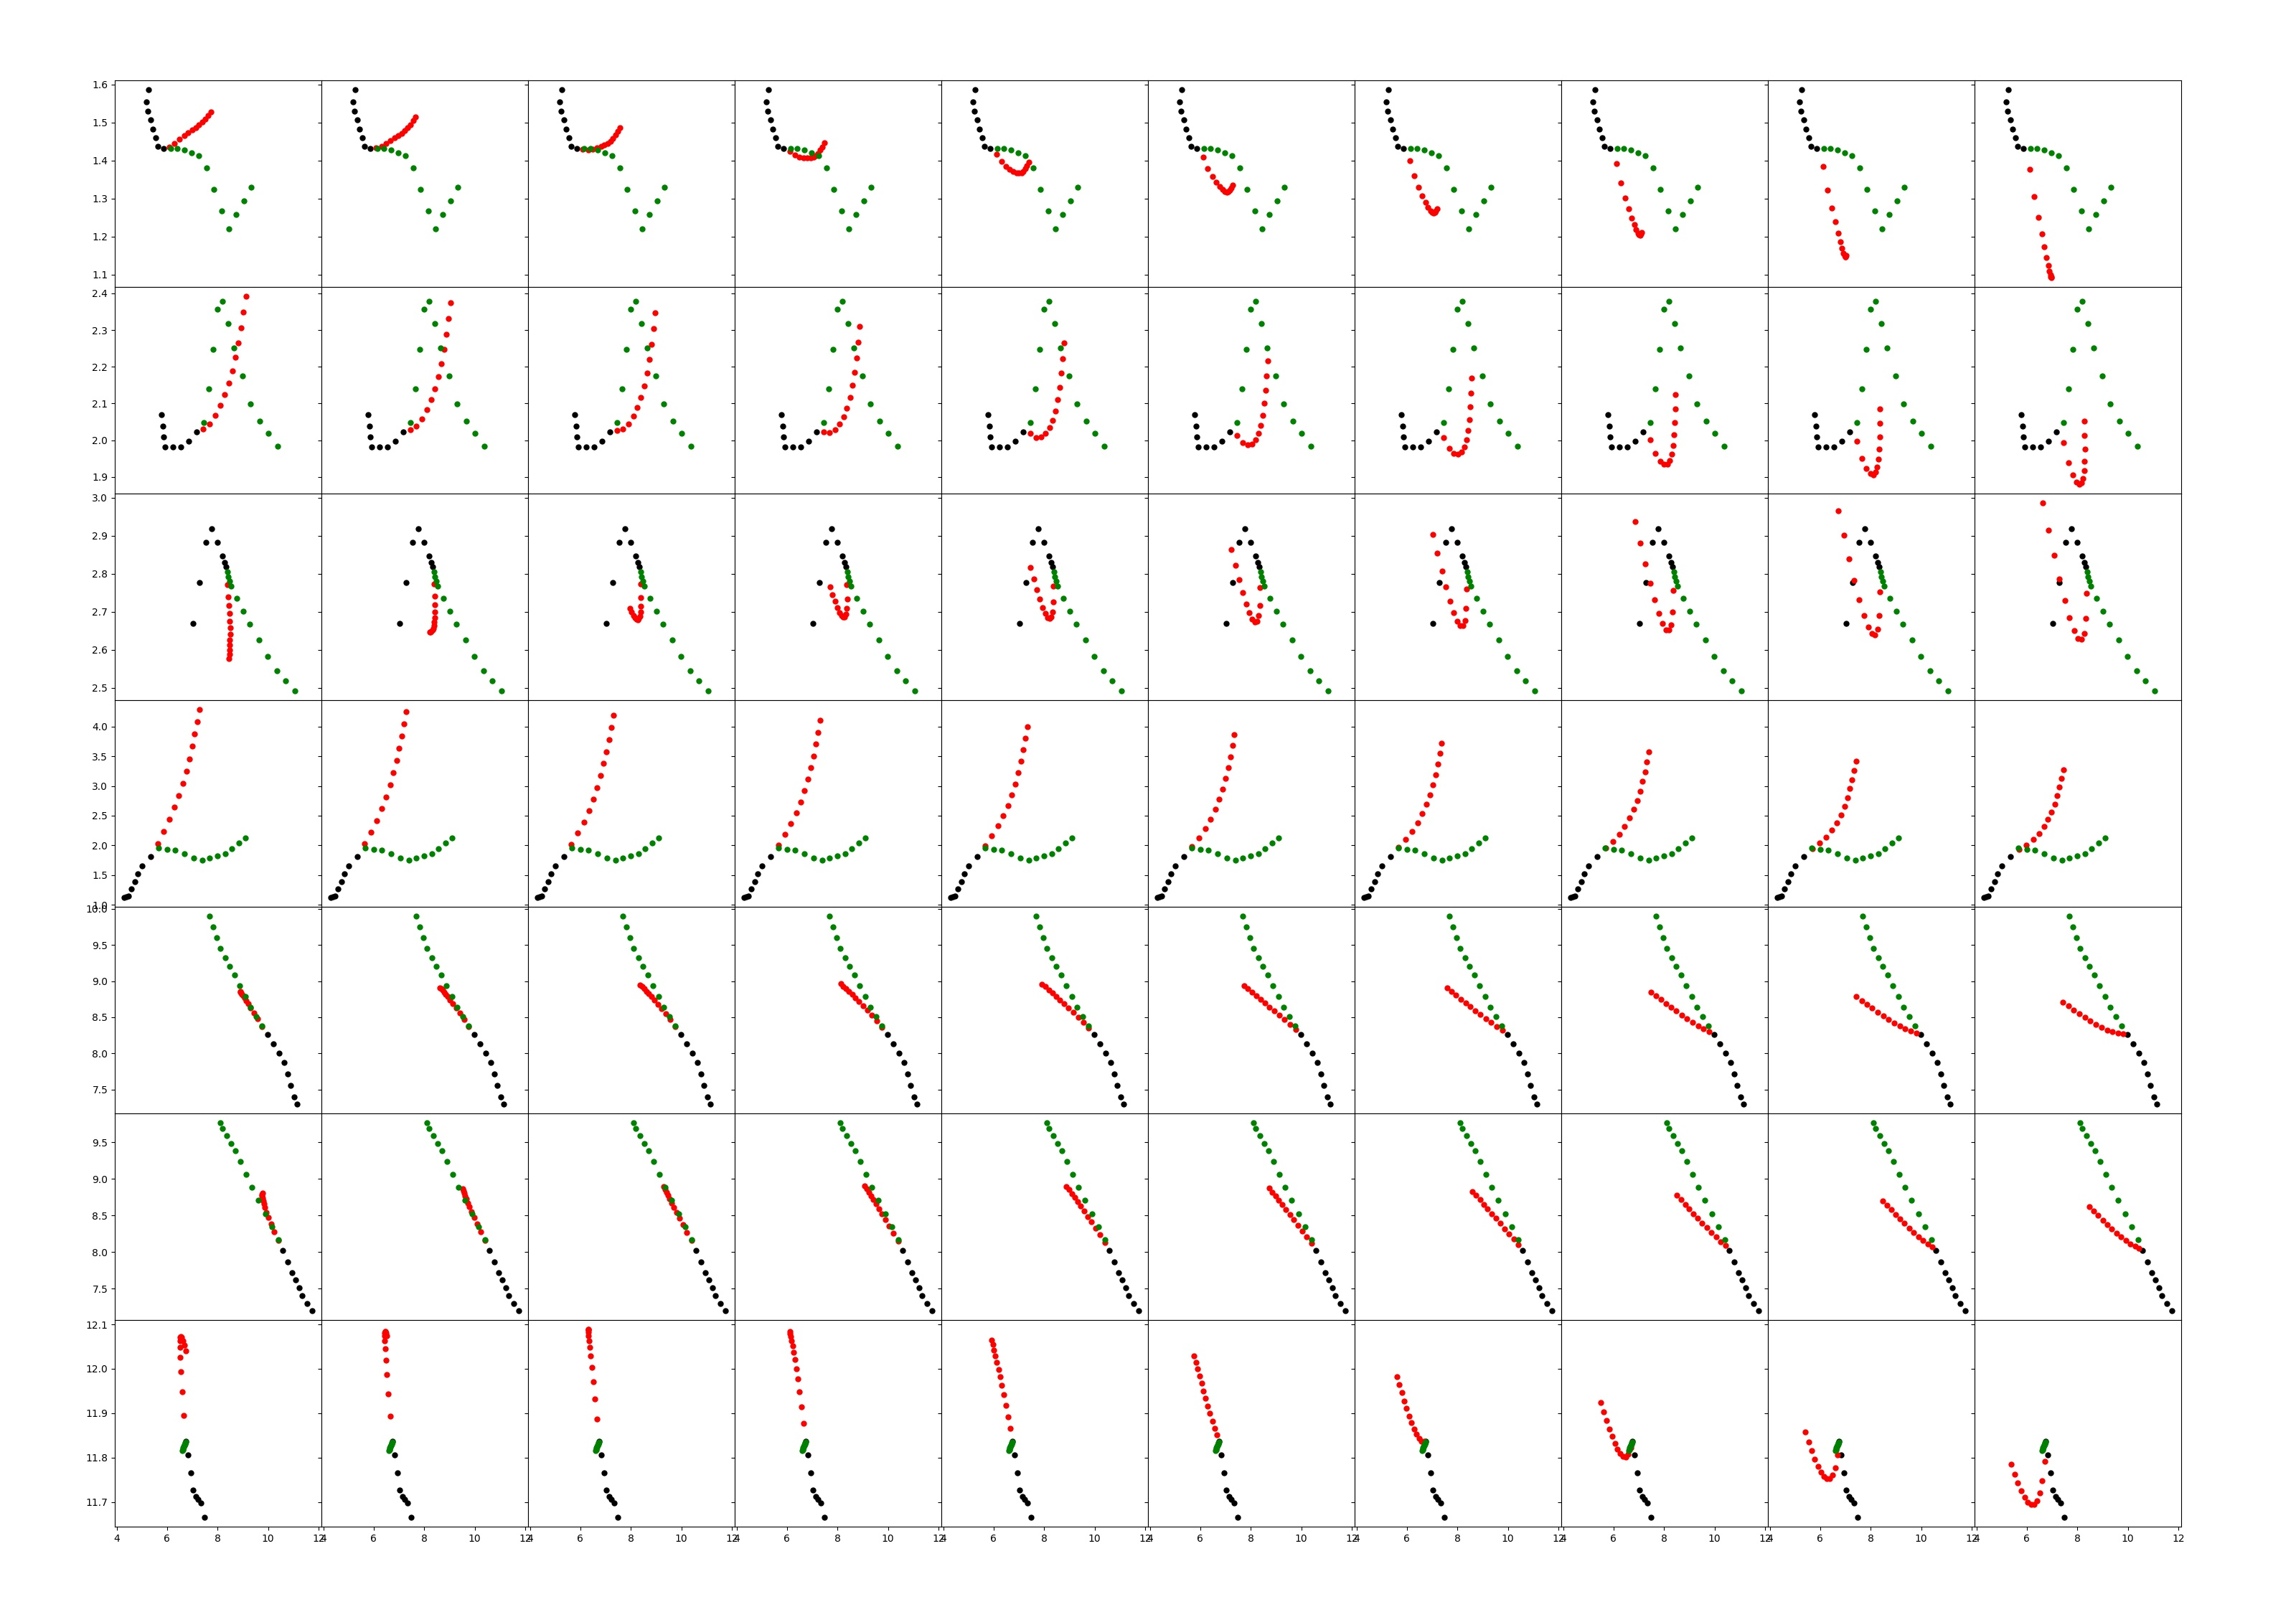
\includegraphics[width=0.8\textwidth]{figures/cont_interpolations_code0_batch2.jpeg}
  \caption{Latent traversals of the continuous latent code for model UNIV\_12. \normalfont{The x-axis is the traversals of range $(-2, 2)$, The y-axis is the different samples. The black dots show the observed trajectory, the green dots show the ground true of the next 12 steps trajectory, the red dots show the prediction of our model.}}{Increasing the code from -2 to 2, the trajectory seems to move downwards. However, this is not always the case, for example the change is not so obvious for the $5^{\text{th}}$ and $6^{\text{th}}$ samples.}
  \Description{latent traversals disc code}
  \label{cont_code}
\end{figure*}

We first evaluate the performance of the modified model and compare it with other models. Table~\ref{table:adefde} shows the results of our modified model under one categorical latent code and one continuous latent codes. We trained our model with the following hyperparameters: one categorical latent code with three dimensions, one continuous latent code, the weight of infomation loss range from $0.03$ to $0.1$. The other hyperparameters are the same as the hyperparameters of SGAN model we trained. It can be seen that our results are slightly better than the SGAN model. This may be due to the fact that the additional InfoGAN slightly helps to structure the latent space.

To observe the performance of untangling, we plotted the latent traversal for different samples. Figure~\ref{disc_code} shows the latent traversal of the categorical latent code. It is noted that the interpretation of the discrete codes is difficult. This is not surprising, probably because it is not easy to describe categorical information in a two-dimensional coordinate space.

Figure~\ref{cont_code} shows the traversals of the continuous code. It can be seen that there is a roughly consistent variation in the continuous latent codes across most of the samples. (e.g. moving the trajectory to downwards, but that is not always the case. With the code increase, the direction of the trajectory slightly change). We must point out that the information loss for the continuous code cannot decrease to a low level, as shown in Figure. This indicates that the information between the latent code and the generated samples has not been maximized, so the latent space is still entangled. This might also explains the fact that our InfoGAN has only a slight improvement in ADE/FDE.


In addition, we point out that the InfoGAN we added to SGAN is hard to train. Unlike the information loss that decreases quickly as mentioned in the InfoGAN, the information loss of continuous code may not change for some information loss weights. We found that for continuous codes, the infomation loss weight that enables the loss decrease and relatively fast learning  range from $0.03$ to $0.1$. A cosine annealing schedule (with restart) for information loss weights may be helpful.

\begin{figure*}[t]
  \centering
  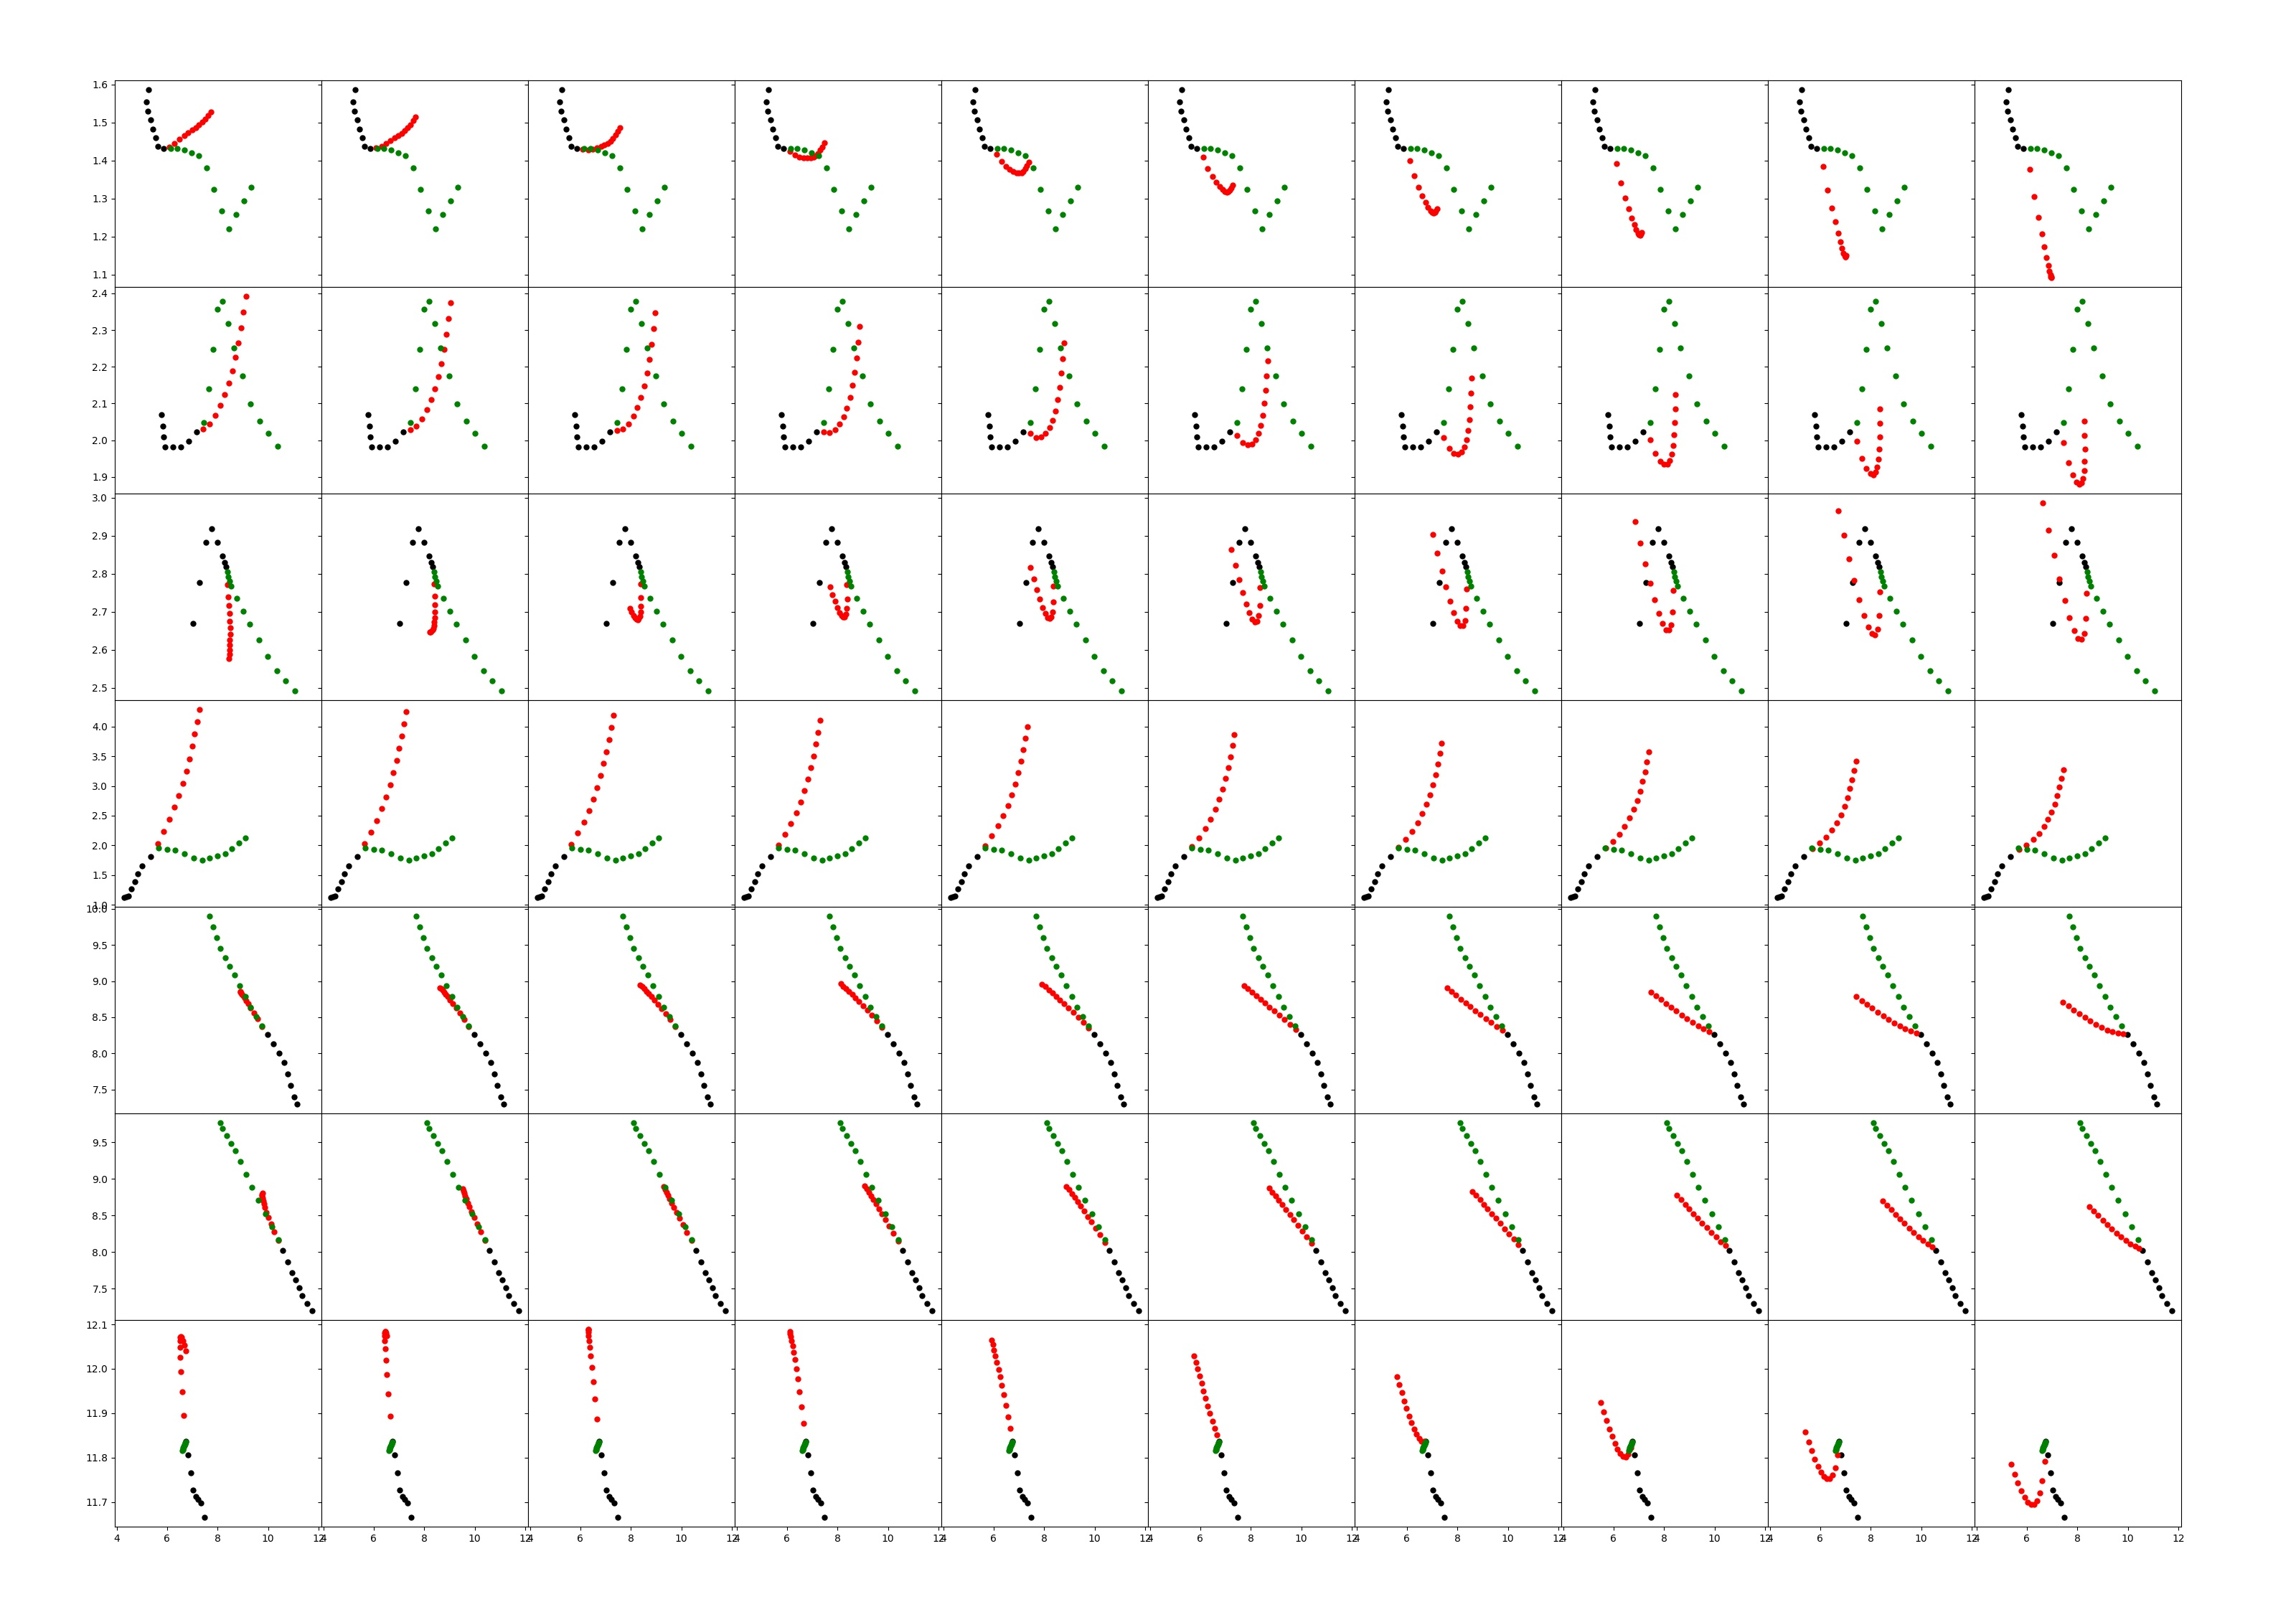
\includegraphics[width=0.7\textwidth]{figures/cont_interpolations_code0_batch2.jpeg}
  \caption{Latent traversals of the continuous latent code 0 for model UNIV\_12 with regularization. \normalfont{The plot style follows Figure \ref{cont_code} (i.e. the meaning of x-axis, y-axis and colors). }}
  \Description{latent traversals cont code 0}
  \label{cont_code_0}

  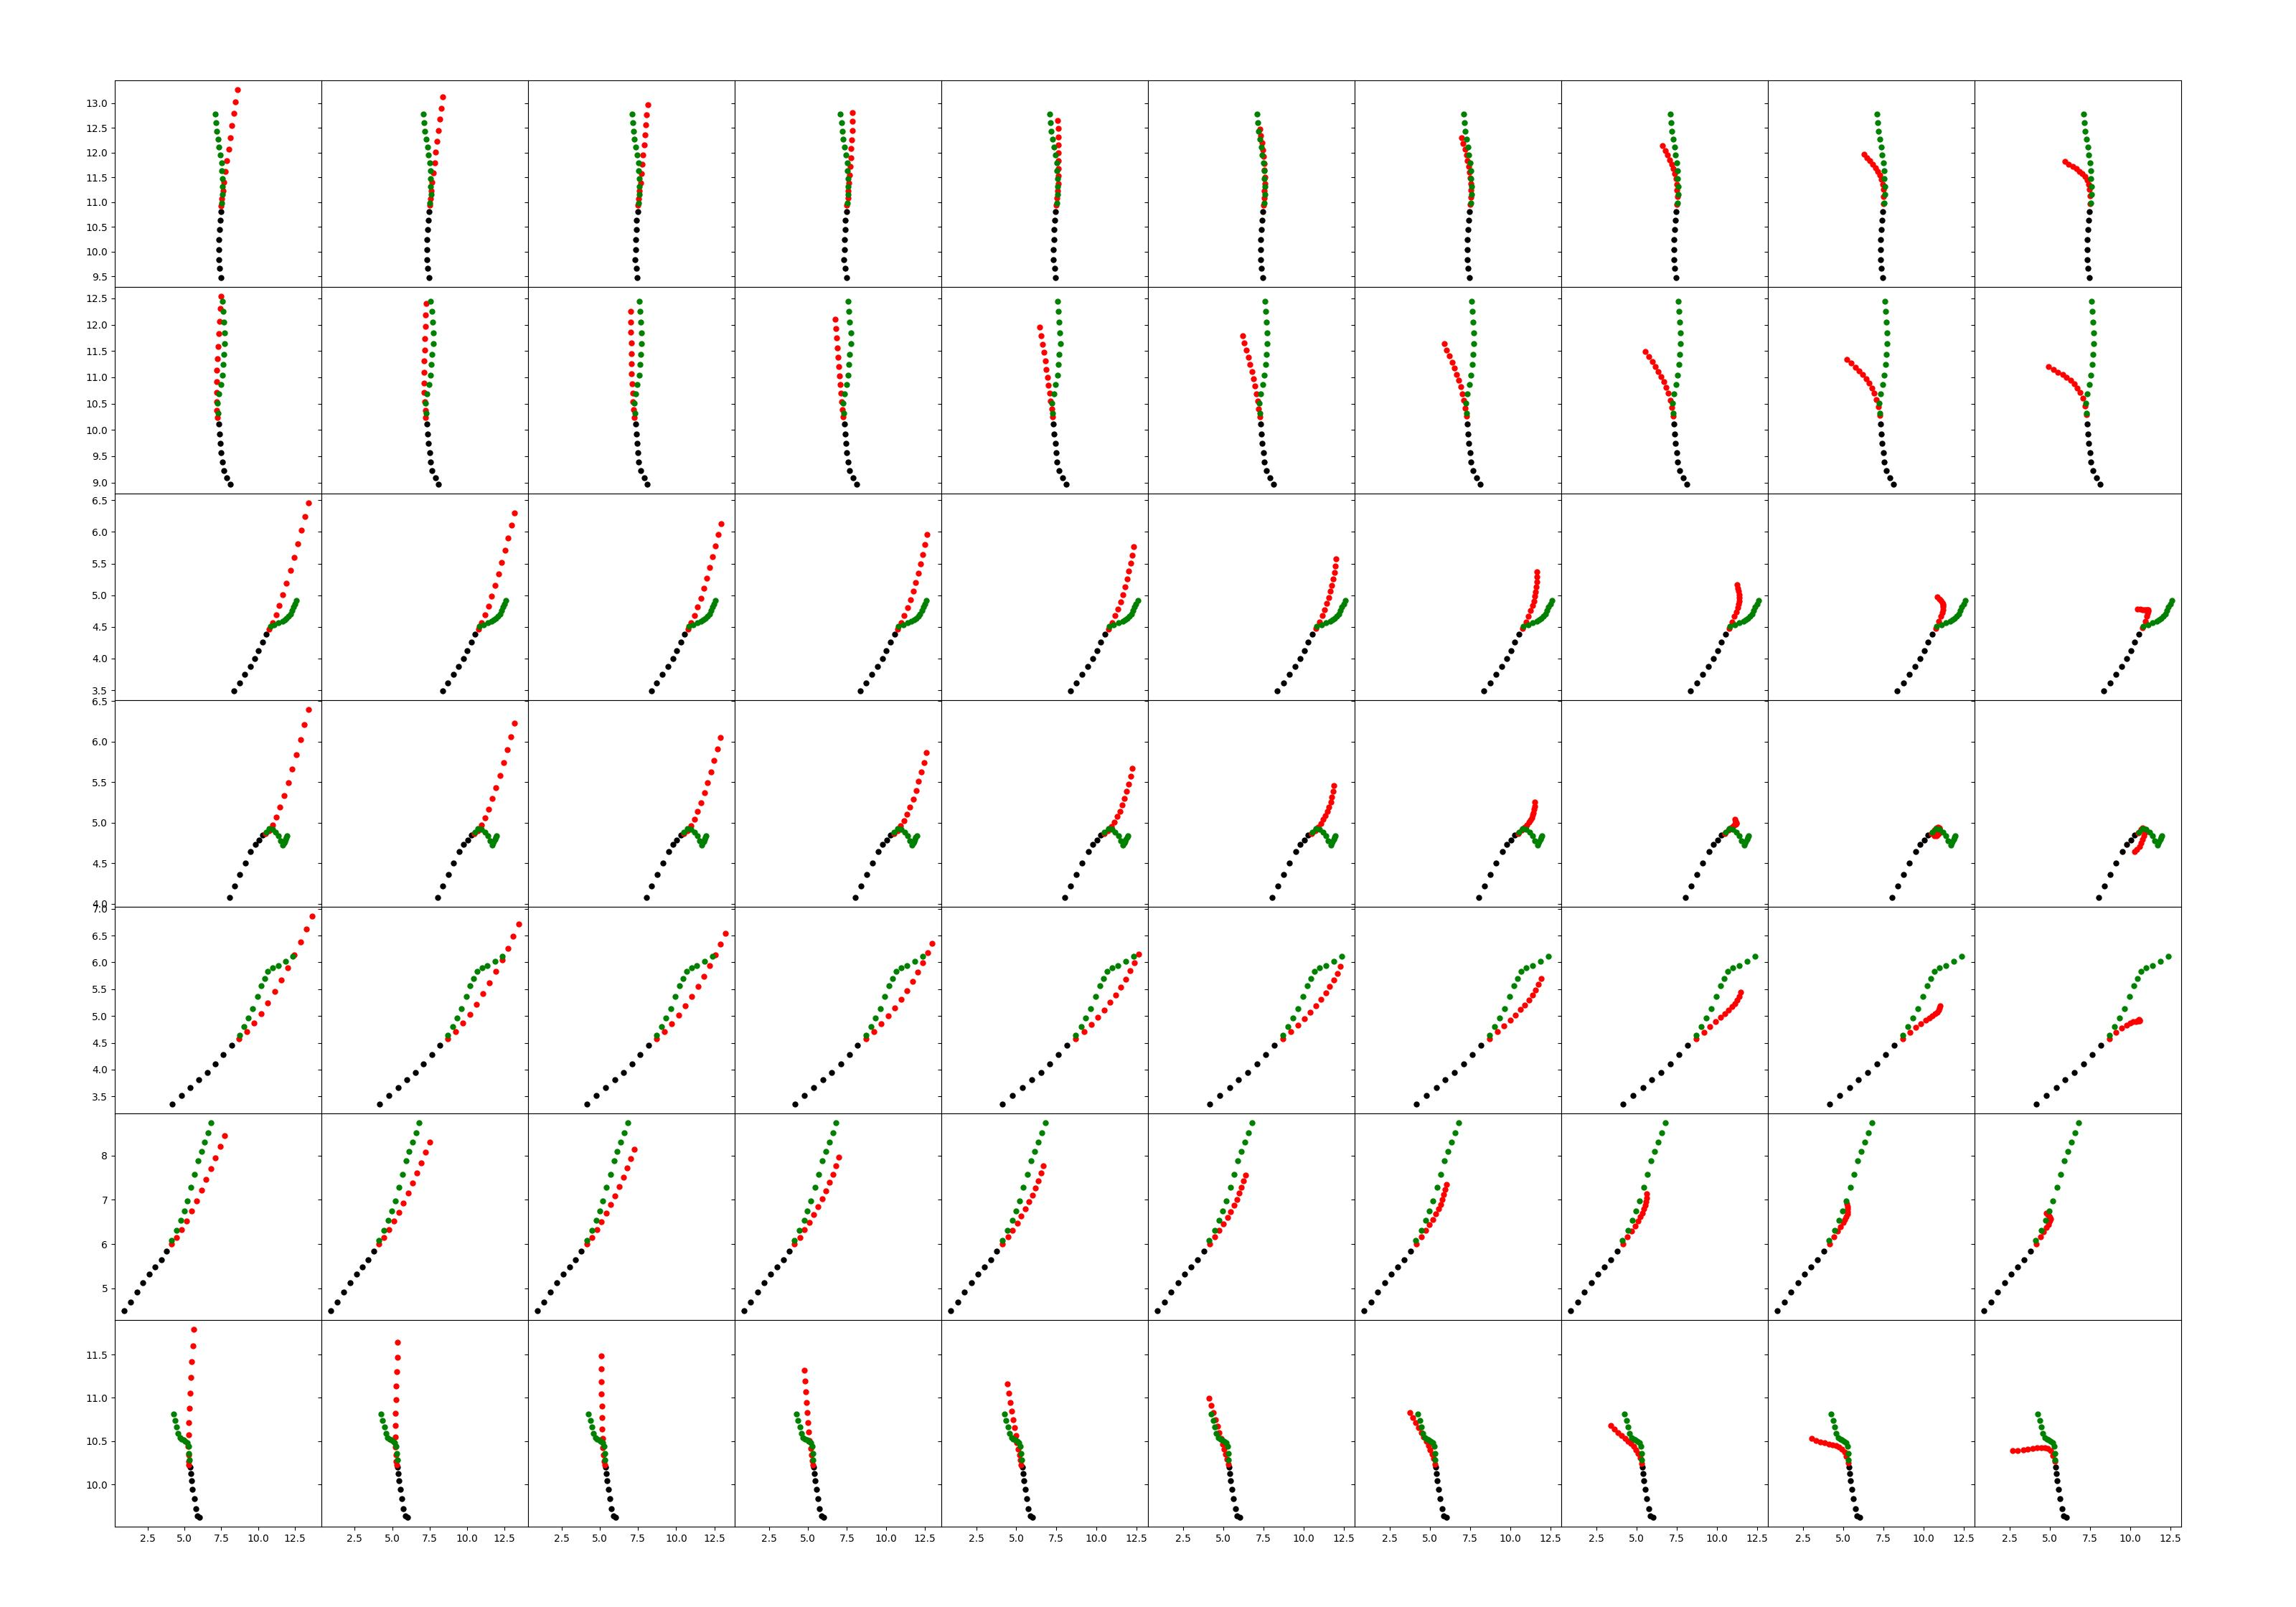
\includegraphics[width=0.7\textwidth]{figures/reg_cont_interpolations_code1_batch1.jpeg}
  \caption{Latent traversals of the continuous latent code 1 for model UNIV\_12 with regularization. \normalfont{The plot style follows Figure \ref{cont_code} (i.e. the meaning of x-axis, y-axis and colors). }}
  {The change induced by code 1 is not so consistent. }
  \Description{latent traversals cont code 1}
  \label{cont_code_1}
\end{figure*}

\subsubsection{Impact of Regularization}
\hfill \\

To disentangle the latent space, we add a regularization constraint that the generated sample changes contributed by one code should be uncorrelated with the changes contributed by the other code. That is, the two codes should be disentangled. We train two continuous code. Figure~\ref{cont_code_0} shows the traversal of continuous latent codes with regularization, it seems that it always make the trajectory to downside. But for code 1, as shown in Figure~\ref{cont_code_1}, it was observed that the code changes were not consistent across samples, so the code remained entangled. The reason behind this may be that the orthogonality of the variation between the two trajectory embeddings may not imply that the variation between the generated samples is orthogonal. Let us take the example of the orthogonal variables in the two coordinate dimensional spaces, i.e., velocity and direction., the changes in trajectory embedding caused by these two factors may not be orthogonal. The other speculation is that the data set is not sufficiently distributed. For example, in most cases, people walk at the same speed, with only a very small sample of high and low speeds.

In addition, we found that adding this regularization reduces the learning time of InfoGAN (information loss can be reduced faster). However, it increases the learning time of SGAN (SGAN loss is reduced slower than before). We found that to get the same performance as before, we need to train for a longer time. But with longer time, we may get better performance than before, while before, longer training time does not increase performance.

\subsection{Conclusion}
To build a controllable generative model to predict trajectories, we added InfoGAN to the Social GAN model. We show that InfoGAN can actually disentangle the latent space, but that is not always the case. This may be an open question, and we have not investigated it in our study. One guess could be that there is not enough signal in the dataset. Futher, we added orthogonality constraints on the sample variation induced by different codes. Although it did help in our case, this approach may be applicable to latent code disentanglement in other tasks (e.g., image generation) and needs to be explored. Finally, there are many ways to constrain the changes caused by the latent codes and then distinguish the factor that affects the human motion trajectory. In future work, we can explore other ways to constrain the changes of the two codes to make them unrelated.


%%
%% The next two lines define the bibliography style to be used, and
%% the bibliography file.
\bibliographystyle{ACM-Reference-Format}
\bibliography{report}

%%
%% If your work has an appendix, this is the place to put it.
\appendix


\end{document}
